% Section 11: Experiments and results (Writer W draft, revised by Opus A after review, 2026-11-21).
% Authority for every number: builds/moc_extensions_plan_2026-11-21/opus_b/e*/result.json.
\section{Experiments and results}\label{sec:experiments}

\textbf{Pre-registration.} Each experiment had a hypothesis and an acceptance
criterion registered before it ran, and recorded statuses are never revised.

\textbf{Follow-ups} are separate records and cannot change a parent's status: DIAGNOSTIC
(script-local harness or variant: E02b, E07b, E09b, E09c, E10b, E11b,
E12-diag-branch), POST-HOC (chosen after the parent result: E05b, E12b) and report-only
(E08b).

\textbf{Evidence classes,} as on page~1: numerical verification (exact solution,
limit, or code-to-code agreement of two repository algorithms), benchmark agreement
(published data or an independent external code), or neither. No run is physical
validation, and none changed a production default, tolerance, gate or coefficient.

\textbf{Setting.} Most runs use the t19 pair for Nozzle-B \cite{rao1958}, whose band is
$\max|\Delta M|=8.04\times10^{-4}$, $\max|\Delta\theta|=0.0229^\circ$,
$\max|\Delta(p/p_0)|=7.49\times10^{-5}$ and $|\Delta C_F|/C_F=3.98\times10^{-5}$.
$C_D=\dot m/(\pi\rho^*a^*R_t^2)$ is the start-line discharge coefficient.

{\footnotesize\renewcommand{\LTcaptype}{table}
\setlength{\tabcolsep}{3.5pt}
\renewcommand{\arraystretch}{1.05}
\begin{longtable}{@{}P{0.66in}P{1.36in}P{0.98in}P{1.00in}P{2.36in}@{}}
\caption{Experiment register. Each status is copied verbatim from the record's \texttt{result.json}.}\label{tab:experiments}\\
\toprule
ID & Question & Recorded status & Evidence class & Key numbers\\
\midrule
\endfirsthead
\multicolumn{5}{@{}l}{\textit{Table~\ref{tab:experiments}, continued}}\\
\toprule
ID & Question & Recorded status & Evidence class & Key numbers\\
\midrule
\endhead
\midrule
\multicolumn{5}{r@{}}{\textit{continued on next page}}\\
\endfoot
\bottomrule
\endlastfoot
E01 & Where do the t19 differences concentrate? & PASS & verification & Metrics reproduced (2546 points); RMS/max 0.17 ($\theta$), 0.20 ($M$); hypotheses not supported.\\
E02 & Why do the LEA/TOP length tests fail? & PASS & verification; benchmark agreement & $L/\Rt$ 15.044818739 (rounded) vs 15.000000000 (sharp); 19 of 20 $\tan15^\circ$ sites sharp (11 of 12 in \code{raosim/}).\\
E02b & Does the source's geometry fit LEA better? & PASS-DIAGNOSTIC & neither & $L/\Rt=15.2796$; RMS 0.0714 vs 0.0870 (throat origin); 0.148 vs 0.152 from N.\\
E03 & How large is the local-$\gamma$ error in $\nu$? & PASS & verification (limit); neither & Limit $1.7\times10^{-12}$\,deg; local $\gamma$ 7.32--8.92$^\circ$; fixed $\gamma$ 3.95--13.10$^\circ$.\\
E04 & How far is $C_{F,\mathrm{MOC}}$ from the Q1D closure? & PASS & neither & Ratio 0.9672 ($C_D=1.0075$) vs $\eta_{C_F}$ 0.98--0.99; wall exit $p/p_0$ 0.0465 vs 0.0302.\\
E05 & Does the net converge on exact source flow? & FAIL & verification & Non-monotone in 2 of 4 cases, order 0.76 in a third (exit-lip row); post hoc interior 1.59--1.76.\\
E05b & Does the lip row bias exit functionals? & PASS-DIAGNOSTIC & verification (post hoc) & $15^\circ$: order 1.97--2.02, lip row $\le1.6\,\%$ of error; $25^\circ$ INVALID-AS-ORACLE.\\
E06 & Is the axis limit handled? & PASS & verification & \code{solve_axis_point} order 2.0 ($M$), 3.0 ($x$); 0 zero-radius hits.\\
E07 & Does the net replay the accepted wall? & FAIL-DIAGNOSTIC & verification (code-to-code) & Kernel bit-identical; first post-kernel RRC folds at $x=4.70/4.79\,\Rt$, beyond the exit.\\
E07b & Does an exit-limited march match the BVP? & PASS-DIAGNOSTIC & verification (code-to-code) & 48/64: $|\Delta M|\le2.2\times10^{-4}$, $|\Delta\theta|\le0.0072^\circ$, $|\Delta C_F|/C_F=8.7\times10^{-6}$.\\
E08 & Do separation criteria differ beyond the reserve? & PASS & neither & Incipient $p_0/p_a$ 8.28--9.19 (spread 1.11 $<$ 1.2); Schmucker wall 9.02 vs Q1D 12.98.\\
E08b & Does E08 change on forward-net states? & PASS & neither (report-only) & Changes $\le1.6\times10^{-6}$ (48/64), $\le3.8\times10^{-6}$ (32/48).\\
E09 & Does the corrected KL sign raise residual order? & PASS-DIAGNOSTIC & verification; neither & Slope gain 1.25--1.30; $C_D$ 1.0075 (KL-V0), 0.9968 (KL-V1); replay INCOMPLETE.\\
E09b & Which start-line variant is sound? & PASS-DIAGNOSTIC & neither & Push inactive; $C_D$ KL-V2 1.0068, KL-V3 0.9944; at $n=64$ KL-V1, KL-V2 fail near the axis.\\
E09c & How much does KL-V3 change the replay? & PASS-DIAGNOSTIC & neither & $\Delta M_B=+0.053$; wall $|\Delta M|$ 0.057 (71$\times$), $|\Delta(p/p_0)|$ 0.017 (221$\times$); $\Delta C_F/C_F=-1.22\,\%$ (307$\times$).\\
E10 & Where and why does the TOP net fold? & INCOMPLETE & neither & t01 reproduced; $r/\Rt$ 0.941--0.950 while $x$ drifts 55.3$\to$50.7\,mm.\\
E10b & Do straight-$C^-$ envelopes locate the fold? & PASS-DIAGNOSTIC & neither & No intersection inside the nozzle; wall $M$ 1.868$\to$2.537.\\
E11 & Can the net run a $\delta^*$-displaced wall? & FAIL-FEASIBILITY & neither & All four scales fold inside ($x=1.17$--$0.32\,\Rt$).\\
E11b & Does an effective throat make it feasible? & FAIL-FEASIBILITY & neither & $s=1$ completes ($\Delta C_F=+0.0001$ effective, $-0.0053$ geometric throat); $s=2$ folds.\\
E12 & Are kernel derivatives smooth between events? & FAIL & verification & Taylor slopes 2.00--2.09; 48 ($J_1$), 54 ($J_3$) jumps without a row-count change.\\
E12-diag-\allowbreak branch & Which branch switches explain the jumps? & FAIL-DIAGNOSTIC & verification & 12 TH3-clamp switches; 36 ($J_1$), 42 ($J_3$) unexplained.\\
E12b & Do Taylor tests pass at event-free points? & FAIL (POST-HOC) & verification (post hoc) & $J_2$, $J_3$ slope 2.000; $J_1$ forward fit spans 1 decade (fail); backward passes at 2 of 3 points; 70 guards.\\
E13 & Can a deterministic OpenFOAM case set be written? & PASS & verification (files only) & 31\,456/125\,824/503\,296 cells; static checks pass; 12 entries UNVERIFIED.\\
E14 & Can Farley--Campbell data serve as a benchmark? & INFEASIBLE & benchmark (not reached) & No tabulated wall; 8/10-streamline contours with BL correction; pressures only against $A/A_{cr}$.\\
\end{longtable}
}

\subsection{Verification}\label{sec:exp-verification}
\textbf{E01} verifies one case's resolution, but gives no observed order.

\textbf{E05, E05b, E06} are discussed in Section~\ref{sec:verification}. E05 is FAIL:
in two cases the maximum error is non-monotone, and a third converges at order 0.76
(Fig.~\ref{fig:e05}). E05b's functional orders and the excluded-row orders are post
hoc.

\textbf{E07 and E07b.} E07 is FAIL-DIAGNOSTIC: the production net folds at
$x=4.70$--$4.79\,\Rt$, outside the nozzle. The E07b harness truncates each RRC beyond
the exit. It was bit-identical to production on the E05 oracle (269 nodes), and it
matches the BVP within the pre-declared thresholds (Fig.~\ref{fig:e07b}). Both
algorithms share the KL start line.

\begin{figure}[htbp]
\centering
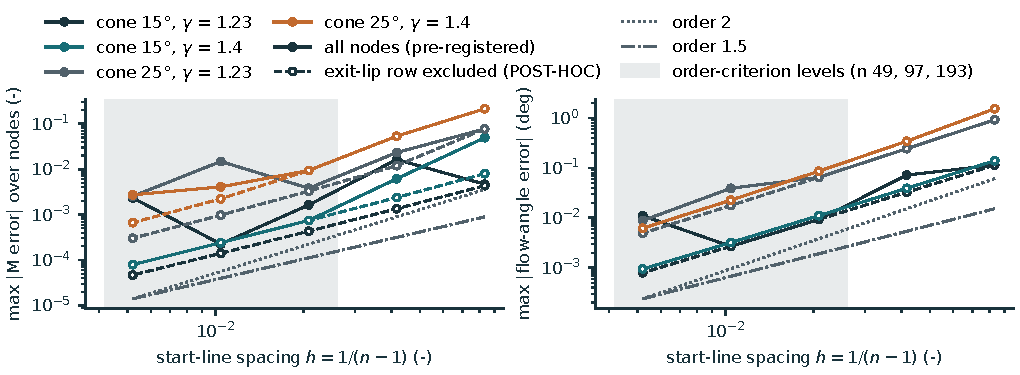
\includegraphics[width=\linewidth]{figures/e05_convergence_mach.pdf}
\caption{E05: production bounded net against exact source flow in cones. (a)~Maximum
Mach error over all nodes against start-line spacing $h$ for the four cone/$\gamma$
cases ($n=13$--193). Solid: all-node series, the pre-registered FAIL basis. Dashed
with open markers: the exit-lip row excluded (POST-HOC). Reference slopes of orders 2
and 1.5; grey band: criterion levels $n=49$, 97, 193. (b)~The same for the maximum
$\theta$ error (deg). Evidence class: verification. Recorded status: FAIL. Script:
\protect\code{scripts/moc_ext_e05_source_flow_oracle.py}.}
\label{fig:e05}
\end{figure}

\begin{figure}[htbp]
\centering
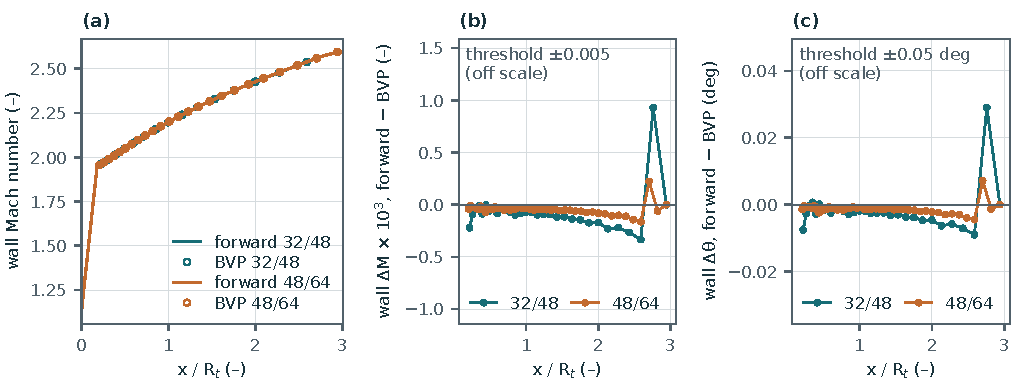
\includegraphics[width=\linewidth]{figures/e07b_exit_limited_replay.pdf}
\caption{E07b: exit-limited replay of the accepted Nozzle-B walls. (a)~Wall Mach
against $x/\Rt$: forward net (lines) and BVP wall nodes (circles), 32/48 and 48/64.
(b)~Wall $\Delta M\times10^3$ and (c)~wall $\Delta\theta$ (deg), forward minus BVP;
the diagnostic thresholds $\pm0.005$ and $\pm0.05^\circ$ are off scale. Evidence
class: verification (code-to-code; both algorithms share the KL start line). Recorded
status: PASS-DIAGNOSTIC. Script: \protect\code{scripts/moc_ext_e07b_exit_limited_replay.py}.}
\label{fig:e07b}
\end{figure}

\subsection{Transonic start line}\label{sec:exp-startline}
\textbf{E09, E09b, E09c} are discussed in Section~\ref{sec:kl} and shown in
Figs.~\ref{fig:e09} and~\ref{fig:e09c}. E09's replay part is INCOMPLETE, because no
variant reached the exit in the production net. E09c is a forward replay on the
KL-V0-optimised wall, not a corrected design, and D-K0-BVP is not approved (D10).

\begin{figure}[htbp]
\centering
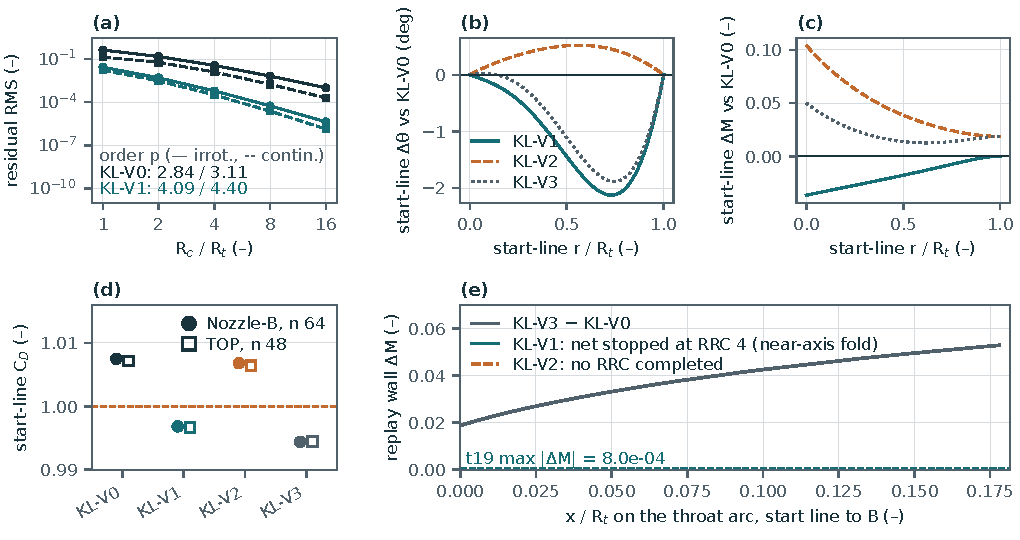
\includegraphics[width=\linewidth]{figures/e09_kl_variants.pdf}
\caption{E09: KL start-line variants (DIAGNOSTIC). (a)~Series-residual RMS against
$R_c/R_t$ at $\gamma=1.23$, for irrotationality and continuity; fitted orders 2.84/3.11
(KL-V0) and 4.09/4.40 (KL-V1). (b, c)~Start-line $\Delta\theta$ and $\Delta M$ relative
to KL-V0 against $r/\Rt$ for KL-V1 to KL-V3 (Nozzle-B, $R_u/R_t=1.5$, $n=64$).
(d)~$C_D$ by variant (Nozzle-B $n=64$; TOP $\gamma=1.2$, $n=48$). (e)~Forward-replay
wall $\Delta M$, KL-V3 minus KL-V0, along the throat arc to B on the 48/64 wall;
KL-V1 stopped at RRC~4 and KL-V2 completed no RRC; dashed: t19 maximum
$|\Delta M|=8.0\times10^{-4}$. Evidence class: verification (a); neither (b--e).
Recorded status: PASS-DIAGNOSTIC. Script: \protect\code{scripts/moc_ext_e09_kl_variants.py}.}
\label{fig:e09}
\end{figure}

\begin{figure}[htbp]
\centering
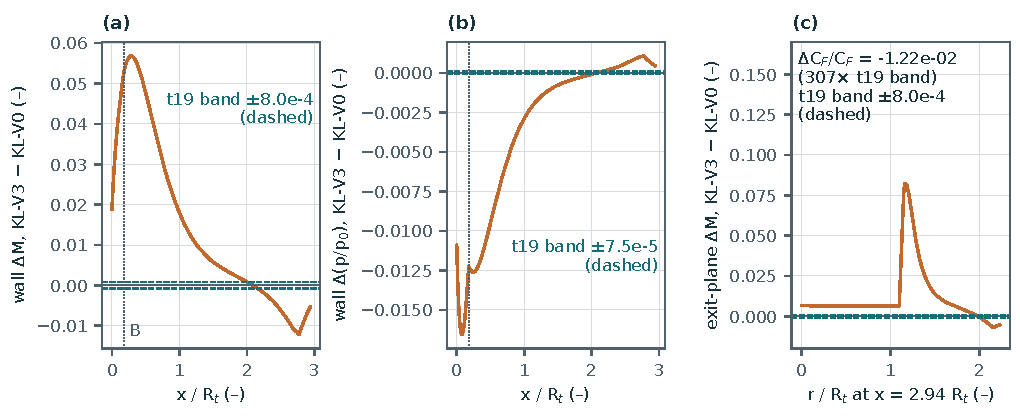
\includegraphics[width=\linewidth]{figures/e09c_k0b_replay.pdf}
\caption{E09c: KL-V3 replay of the accepted 48/64 Nozzle-B wall in the E07b harness.
(a)~Wall $\Delta M$, KL-V3 minus KL-V0, against $x/\Rt$, with B marked and the t19 band
$\pm8.0\times10^{-4}$. (b)~Wall $\Delta(p/p_0)$, band $\pm7.5\times10^{-5}$.
(c)~Exit-plane $\Delta M$ against $r/\Rt$ at $x=2.94\,\Rt$;
$\Delta C_F/C_F=-1.22\times10^{-2}$ (307 times the band). This is a forward replay on
the KL-V0-optimised wall, not a corrected design. Evidence class: neither
(diagnostic). Recorded status: PASS-DIAGNOSTIC. Script:
\protect\code{scripts/moc_ext_e09c_k0b_replay.py}.}
\label{fig:e09c}
\end{figure}

\subsection{Thermodynamics, geometry and separation}\label{sec:exp-thermo}\label{sec:exp-geometry}\label{sec:exp-separation}
E03's reference is the thermally perfect integral
\cite[Eqs.~4.35--4.36, PDF p.~186]{anderson}, \cite[Eq.~200, thermally perfect;
Eq.~199 general]{ames1953}. It passes the constant-$c_p$ limit, and the substitution
errors reject local-$\gamma$ use (Section~\ref{sec:g1}). E02, E02b and E04 are in
Section~\ref{sec:geometry-arch}. E08 and E08b are in Section~\ref{sec:g3}; they are
screening comparisons on an inviscid vacuum wall and say nothing about which criterion
is right.

\subsection{Shocks, viscous coupling and derivatives}\label{sec:exp-shocks}\label{sec:exp-viscous}\label{sec:exp-derivatives}
\textbf{E10 and E10b.} E10 is INCOMPLETE: the net stores no bell wall state, so H2 and
the envelope part of H3 were not evaluated (Fig.~\ref{fig:e10}). The straight-shock
bound $p_{02}/p_{01}=0.917$ cannot be tested, because no open numeric TOP
internal-shock data were found \cite[Sec.~3.5, PDF p.~26]{ostlund}, \cite{ruf2010}.

E10b accepted 136 bell wall nodes upstream of the first reversed cell. Neither their
straight $C^-$ nor the planar simple-wave envelope (Prandtl--Meyer relation
\cite[Eq.~4.44, PDF p.~187]{anderson}; envelope criterion
\cite[Secs.~24--25]{courant1944}) intersects inside the nozzle, so H2 is not supported.

\textbf{E11 and E11b} are FAIL-FEASIBILITY (Section~\ref{sec:g3}).

\textbf{E12, E12-diag-branch, E12b} (Fig.~\ref{fig:e12}). The Taylor test passes inside
event-free windows, but 36 ($J_1$) and 42 ($J_3$) jumps remain unexplained. In E12b,
the forward $J_1$ fit spans only one decade at all three points. The backward fit
passes (slope 1.988) at 27.2975$^\circ$ and 27.7975$^\circ$, but spans one decade at
28.2975$^\circ$.

\begin{figure}[htbp]
\centering
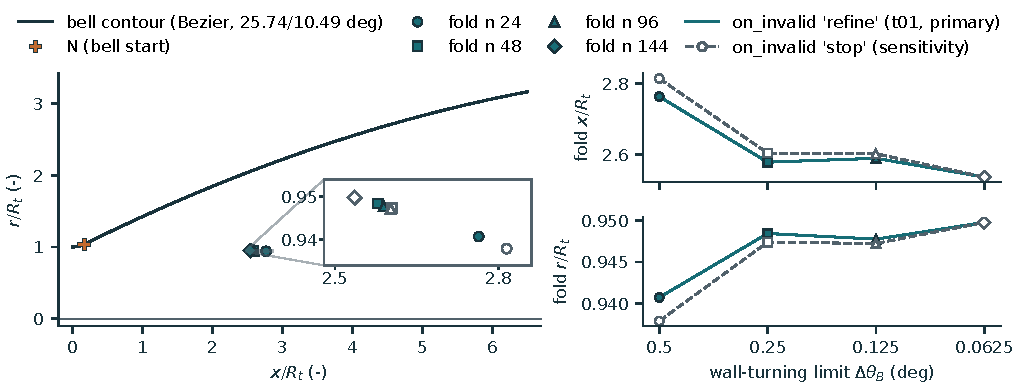
\includegraphics[width=\linewidth]{figures/e10_fold_envelope.pdf}
\caption{E10: fold on the current-chart TOP bell ($\Rt=20$\,mm, $\varepsilon=10$, 80\,\%,
$\gamma=1.2$). (a)~Bell contour (geometry from \protect\code{bell_nozzle_contour},
not a MOC run) with N and the four fold points of the primary
\protect\code{on_invalid='refine'} runs; the inset zooms on the fold cluster, with the
'stop' folds as open markers. (b)~Fold $x/\Rt$ and (c)~fold $r/\Rt$ against the
wall-turning limit (0.5 to $0.0625^\circ$, $n=24$ to 144); 'refine' solid, 'stop'
dashed. Evidence class: neither. Recorded status: INCOMPLETE. Script:
\protect\code{scripts/moc_ext_e10_top_fold_envelope.py}.}
\label{fig:e10}
\end{figure}

\begin{figure}[htbp]
\centering
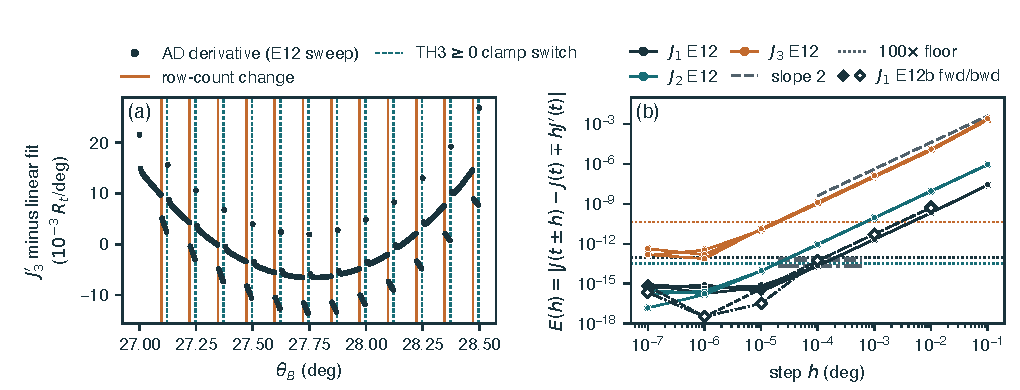
\includegraphics[width=\linewidth]{figures/e12_taylor_events.pdf}
\caption{E12: JAX throat kernel on the Nozzle-B arc. (a)~$\theta_B$ sweep 27.0--28.5$^\circ$
(301 points): $\dd J_3/\dd\theta_B$ minus its linear fit ($10^{-3}\,\Rt$/deg); solid
lines mark the 12 row-count changes and dashed lines the 12 TH3-clamp switches.
(b)~Taylor remainder $E(h)$ against $h$. Panel (b) mixes pre-registered E12 data
(solid: forward remainders of $J_1$, $J_2$, $J_3$ at 27.23, 27.73 and 28.23$^\circ$;
dotted: each output's 100$\times$ noise floor) with post-hoc E12b data ($J_1$ at
27.7975$^\circ$: forward dashed, backward dash-dot), distinguished by line style;
slope-2 reference. Evidence class: verification. Recorded status: E12 FAIL; E12b FAIL
(POST-HOC). Script: \protect\code{scripts/moc_ext_e12_jax_kernel_taylor.py}.}
\label{fig:e12}
\end{figure}

\subsection{CFD case writer and benchmark data}\label{sec:exp-cfd}\label{sec:exp-benchmark}
\textbf{E13} is a prototype pending D1; nothing about the flow is established until the
user runs the cases (Section~\ref{sec:cfd}).

\textbf{E14} is INFEASIBLE. Farley and Campbell's contours are 8/10 streamlines of
Clippinger's sharp-throat nozzles with boundary-layer corrections
\cite[PDF pp.~4, 19]{farley1960}. The forward net cannot regenerate the corrected walls
from published data without improvising the throat. Their wall pressures are plotted
only against $A/A_{cr}$ \cite[Fig.~10, PDF pp.~26--27]{farley1960}.
